\documentclass{ximera}

\input{../../preamble.tex}

\author{Ivo Terek}
\license{Creative Commons Attribution-ShareAlike 4.0 International License}

%\outcome{Calculating the rate of change.}
%\outcome{Discuss the meaning of antiderivatives of a position function.}

\begin{document}
\begin{exercise}



If the graph of $y=f(x) = x\sin(x)$ is given in black below (namely, the only one below with $f(0)=0$), which of the following graphs could be the graph of $y = f(x-2)$?
  \begin{image}
 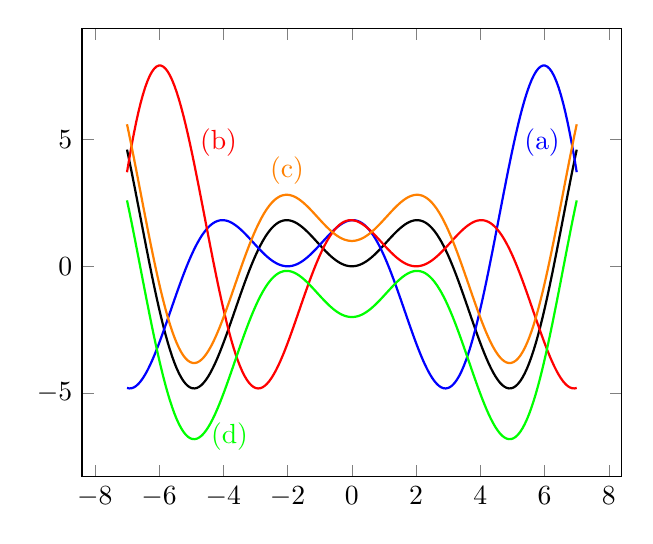
\begin{tikzpicture}
   \begin{axis}
     \addplot[samples=200,thick, domain=-7:7]{x*sin(deg(x))};
     \addplot[samples=200,thick,domain=-7:7, color=blue]{(x+2)*sin(deg(x+2))} node[pos=0.8,right]{\text{(a)}};
     \addplot[samples=200,thick,domain=-7:7, color=red]{(x-2)*sin(deg(x-2))} node[pos=0.2,right]{\text{(b)}};
     \addplot[samples=200,thick,domain=-7:7, color=orange]{x*sin(deg(x)) + 1} node[pos=0.43,above]{\text{(c)}};
     \addplot[samples=200,thick,domain=-7:7, color=green]{x*sin(deg(x))-2} node[pos=0.25,right]{\text{(d)}}; 
   \end{axis}
 \end{tikzpicture}
 \end{image}

\begin{multipleChoice}
  \choice{Blue graph}
  \choice[correct]{Red graph}
  \choice{Orange graph}
  \choice{Green graph}
\end{multipleChoice}

\end{exercise}
\end{document}
